\section{Subject: Specification and Implementation of Distributed Systems}
\label{sec:subject}

The subject of our formalization is a part of the material from the \textit{Specification and Implementation of Distributed System} course taught at ELTE. The main goal was following the official notes of the subject\cite{hz-orsi} as closely as possible, but since the code needed to be more precise than written definitions, some constructs were altered. The system extends a relational model defined in \cite{fothi-prog} which itself is built upon Hoare-logic \cite{hoare1978proof}\cite{hoare-logic}, more specifically concurrent Hoare-logic\cite{Lamport1980}. Proofs for sequential programs are handled using pre- and postconditions with the devices provided by first order logic. This is expanded to parallel execution in a similar fashion to UNITY. Abstract programs are formalized through a set of conditional assignments the execution of which are represented as a list of state transitions that can be considered as trees, which results in a branching-time temporal logic \cite{emerson1988branching} (more specifically computation tree logic) like system.

An abstract program as defined by this system can be thought of as an initialization and a set of further conditional instructions. These are then selected randomly and if their condition is satisfied in the current program state, they are executed. This can be done in any arbitrary order, their behaviour stays the same if the scheduling is impartial. The execution units running such a program can be thought of as processing cores, or even several computers working together in a cluster.

\begin{definition}{Interleaving semantics}
\label{def:interleaving-semantics}
In a model that conforms to interleaving semantics, for every valid parallel execution, there also exists a linear execution path of the same instructions, that achieves equivalent results.
\end{definition}

\begin{definition}{Impartial Scheduling}
\label{def:impartial-scheduling}
A scheduling is called impartial if it ensures that running the program indefinitely will result in the selection of each and every conditional instruction infinitely many times.
\end{definition}

After laying down the foundation for constructing programs and reasoning about their behavior, the subject introduces a formal concept of task specification and then defines the correctness of a program by proving that it adheres to those constraints posed by the specification. We iterate on these constructions and implement them, so the verification of the adherence can be done on the computer, thus avoiding potential human errors that can occur while carrying out such a process on paper.

There are multiple ways, in which said correctness of a program can be shown. Simply giving a proof, that all the imposed criteria are held is always sufficient, but gets inconvenient for larger programs. To avoid the complication of proofs, one can utilize the method of reduction to an already known problem. If there is a recurring pattern, general statements about its behavior can be proven, so that these do not need to be done each and every time the pattern is used. Just showing how the currently examined part of the program corresponds to the pattern is enough instead. Another technique for avoiding repetition and introducing segmentation into proofs to keep their brevity is to construct programs from other smaller programs, by for example taking their union, essentially using them as so called \textit{building blocks}.

\subsection[Mathematical foundation]{Mathematical foundation\protect\footnote{The original model is more general than the one described here, but since our formalization uses functions, that are deterministic, we constrained the ranges of some relations to single values instead of sets.}}

The basics of the material are built on top of a relational model, the development of which originates from the works of Ákos Fóthi\cite{fothi1988mathematical}. This model deals with programs, that operate over a so called \textbf{state space}, which is built as a Cartesian product of the individual sets of possible values for the variables of the program: $A = A_1 \times A_2 \times \ldots \times A_n$. These sets are individually called \textbf{type value sets}. The value of a single variable in a certain state can be accessed by the projection function $v_i : A \to A_i$.

Let $A^*$ denote the finite and $A^\infty$ the infinite sequences made of elements in $A$. The set of all sequences with elements from $A$, that can either be finite or infinite is defined as $A^{**} = A^* \cup A^\infty$.

We call a function a \textit{logical function}, if it maps into the set of Boolean logical values defined as $\mathbb{B} = {true , false}$. A subset of these functions, that not only have $\mathbb{B}$ as their range, but also a state space $A$ as their domain can be called conditions. These have the type $\pi : A \to \mathbb{B}$.

\begin{definition}{Truth set}
\label{def:truth-set}
The subset of the state space in which these conditions are satisfied is often of interest, for this purpose the notion of the \textbf{truth set} of a function is defined as the subset of its domain that it maps to $true$. It is denoted as follows: $\lceil \pi \rceil = \{a \in A \;|\; \pi(a) = true\}$
\end{definition}

\begin{definition}{Implication}
\label{def:implication}
One condition is said to imply another ($P \Rightarrow Q$) if its truth set is subset of the others ($\lceil P \rceil \subset \lceil Q \rceil$).
\end{definition}

Another specific kind of function that operates on states is the so called \textbf{state transition function}. It has the type signature of $A \to A$ and is used to describe the behavior of an instruction. In this model, we consider only a single kind of instruction, namely a generic type of assignment, which is defined in the following way. Given a function for every variable index of the state space, that maps from the entire state space to the type value set of that given variable ($\forall i \in \{1..n\} : F_i : A \to A_i$), combining these into a single function $F = (F_1, \ldots F_n)$ we get a state transition function. Semantically speaking, it describes a parallel assignment, where each variable can have a formula, that may depend on all the other variables (or itself as well), these then are evaluated in the same state and get their new values assigned concurrently to produce a new, updated state.

Such an assignment can be made conditional by pairing it with a logical function. By doing so, we alter its state transition function in a way, that it only applies the changes to the state, if its condition is fulfilled (meaning, that the current state is in its truth set), otherwise it acts as an identity function. With mathematical notation, given $\pi : A \to \mathbb{B}$ as a condition and $F : A \to A$ as an assignment, we get the following conditional state transition function:

\begin{equation}
    F'(a) = 
    \left\{
    	\begin{array}{ll}
    		F(a) & \mbox{if } a \in \lceil \pi \rceil \\
    		a & \mbox{otherwise}
    	\end{array}
    \right.
\end{equation}

A parallel program ($S = (s_0, \{s_1, \ldots, s_m\})$) defined using these constructs consists of a single initialization assignment and a set of conditional assignments to be repeatedly performed later in no particular order. Any requirements that would be posed for their sequentiality need to be encoded into their conditions, which in turn can ensure some sort of a control flow. A parallel program constructed in such a way can be semantically thought of as a relation that maps any state to a branching series of possible successive states (see Figure \ref{fig:branching-execution} as an illustration). If we remove the successively duplicated states from these series by replacing all consecutive repetitions of a single state with only one instance, we get their so-called \textit{reduced} versions. This gives us the type signature $A \times A^{**}$, meaning that for any given state, the program determines the set of possible execution paths, which are either finite (if a program terminates by reaching a fixed point) or infinite (that might represent a continuously running server) series of states.

\begin{figure}[H]
    \centering
    \usetikzlibrary{trees}
% \tikzstyle{level 1}=[level distance=2cm, sibling distance=4cm]
% \tikzstyle{level 2}=[level distance=2cm, sibling distance=1cm]
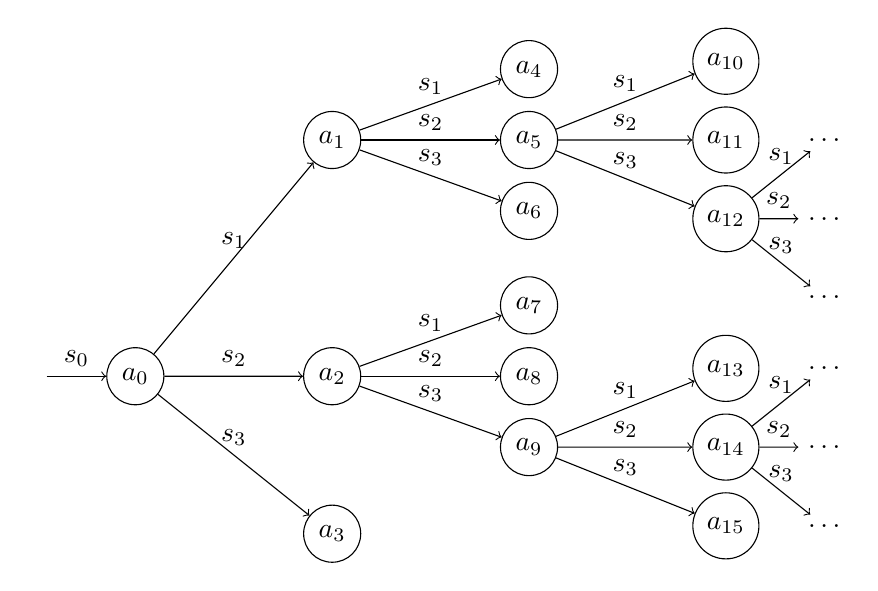
\begin{tikzpicture}[
        grow=right,
        ->,
        % every node/.style={draw,circle},
        state/.style={draw, circle},
        % treenode/.style = {circle, white, draw=black, align=center, inner sep=0pt, text centered, font=\sffamily},
        % thick,
        % Set the overall layout of the tree
        level/.style={level distance=2.5cm},
        level 1/.style={level distance=1.25cm},
        level 2/.style={sibling distance=3cm},
        level 3/.style={sibling distance=0.9cm},
        level 4/.style={sibling distance=1cm},
        level 5/.style={level distance=1.25cm},
        % level/.style={sibling distance = 5cm/#1, level distance = 1.5cm}
    ]
    \node {}
    child {
        node [state] {$a_0$}
        child [sibling distance=2cm] {
            node [state] {$a_3$}
            edge from parent node [above] {$s_3$}
        }
        child {
            node [state] {$a_2$}
            child {
                node [state] {$a_9$}
                child {
                    node [state] {$a_{15}$}
                    edge from parent node [above] {$s_3$}
                }
                child {
                    node [state] {$a_{14}$}
                    child {
                        node {$\ldots$}
                        edge from parent node [above] {$s_3$}
                    }
                    child {
                        node {$\ldots$}
                        edge from parent node [above] {$s_2$}
                    }
                    child {
                        node {$\ldots$}
                        edge from parent node [above] {$s_1$}
                    }
                    edge from parent node [above] {$s_2$}
                }
                child {
                    node [state] {$a_{13}$}
                    edge from parent node [above] {$s_1$}
                }
                edge from parent node [above] {$s_3$}
            }
            child {
                node [state] {$a_8$}
                edge from parent node [above] {$s_2$}
            }
            child {
                node [state] {$a_7$}
                edge from parent node [above] {$s_1$}
            }
            edge from parent node [above] {$s_2$}
        }
        child {
            node [state] {$a_1$}
            child {
                node [state] {$a_6$}
                edge from parent node [above] {$s_3$}
            }
            child {
                node [state] {$a_5$}
                child {
                    node [state] {$a_{12}$}
                                        child {
                        node {$\ldots$}
                        edge from parent node [above] {$s_3$}
                    }
                    child {
                        node {$\ldots$}
                        edge from parent node [above] {$s_2$}
                    }
                    child {
                        node {$\ldots$}
                        edge from parent node [above] {$s_1$}
                    }
                    edge from parent node [above] {$s_3$}
                }
                child {
                    node [state] {$a_{11}$}
                    edge from parent node [above] {$s_2$}
                }
                child {
                    node [state] {$a_{10}$}
                    edge from parent node [above] {$s_1$}
                }
                edge from parent node [above] {$s_2$}
            }
            child {
                node [state] {$a_4$}
                edge from parent node [above] {$s_1$}
            }
            edge from parent node [above] {$s_1$}
        }
        edge from parent node [above] {$s_0$}
    };
\end{tikzpicture}

% \begin{tikzpicture}[
%         ->,
%         every node/.style={draw,circle},
%         % treenode/.style = {circle, white, draw=black, align=center, inner sep=0pt, text centered, font=\sffamily},
%         thick,
%         % Set the overall layout of the tree
%         level/.style={level distance=1.5cm},
%         level 2/.style={sibling distance=2.6cm},
%         level 3/.style={sibling distance=2cm}
%     ]
%     \coordinate
%         child[grow=left]{
%             node {$a_0$}
%             % node [treenode] {$a_0$}
%             edge from parent node [above=3pt] {$s_0$}
%         }
%         % I have to insert a dummy child to get the tree to grow
%         % correctly to the right.
%         child[grow=right, level distance=0pt] {
%         node [above] {$a_1$}
%         child  {
%             child {
%                 child {
%                     node {$\bar{d}$}
%                     edge from parent
%                 }
%                 child {
%                     node {$u$}
%                     edge from parent
%                 }
%                 edge from parent
%             }
%             child {
%                 node {$b$}
%                 edge from parent
%             }
%             edge from parent
%             node [below] {$t$}
%         }
%         child {
%             child {
%                 node {$\bar{b}$}
%                 edge from parent
%             }
%             child {
%                 child {
%                     node {$\bar{v}$}
%                     edge from parent
%                 }
%                 child {
%                     node {$e^{-}$}
%                     edge from parent
%                 }
%                 edge from parent
%             }
%             edge from parent
%             node [above] {$\bar{t}$}
%         }
%     };
% \end{tikzpicture}
    \caption{Branching execution with possible paths, e.g., $(a_0,a_2,a_9,a_{15})$, $(a_0,a_1,a_5,a_{12},...)$.}
    \label{fig:branching-execution}
\end{figure}

By constructing a type of specification that only places constraints on states, we can achieve independence from the actual structure of programs operating on these states. Problems consist of seven so called \textit{Specification Properties}, which are themselves given as relations over the power set of the state space. These provide constraints for the behavior of the program, that will eventually have to satisfy all of them to be considered adherent to the specification and thus solve the problem.

Let $P, Q : A \to \mathbb{B}$, the infix notation $P \Circle Q$ mean $(\lceil P
\rceil , \lceil Q \rceil) \in \Circle$, where $\Circle$ is any of the binary
relations $\rhd, \mapsto, \hookrightarrow$ and for the unary relations $\CIRCLE
\in \{FP, INIT, inv, TERM\}$, let $P \in \CIRCLE$ mean $\lceil P \rceil \in
\CIRCLE$

% They can be classified into four groups:
% Safety properties:
% Progress properties:
Let the following specification properties be proposed:
\begin{itemize}
    \item $\rhd \in \mathcal{P}(\mathcal{P}(A) \times \mathcal{P}(A))$, where $P \rhd Q$ means, that leaving $\lceil P \rceil$ requires going through $\lceil Q \rceil$
    % the truth set of predicate $P$ can only be left by going through the truth set of $Q$
    \item $\mapsto \in \mathcal{P}(\mathcal{P}(A) \times \mathcal{P}(A))$, where $P \mapsto Q$ extends upon $P \rhd Q$ by stating that $\lceil P \rceil$ can indeed be left through $\lceil Q \rceil$, and only through it
    \item $\hookrightarrow \in \mathcal{P}(\mathcal{P}(A) \times
      \mathcal{P}(A))$, where $P \hookrightarrow Q$ states that from every state in the truth set of $P$ we must eventually get to a point in the truth set of $Q$ (formally it is the transitive disjunctive closure (see Definition
      \ref{def:transitive-disjunctive-closure}) of $\mapsto$)
    \item $FP \subseteq \mathcal{P}(A)$ where $P \in FP$ means that if the program has reached a fixed point (meaning, that it can make no further state transitions), then $P$ must be satisfied
    \item $INIT \subseteq \mathcal{P}(A)$, where $P \in INIT$ means that the predicate $P$ is satisfied at the beginning of the program
    \item $inv \subseteq \mathcal{P}(A)$, where $P \in inv$ means that $P$ is satisfied at the beginning of the program and once its truth set has been entered, it cannot be left, thus it is an invariant for the entire program
    \item $TERM \subseteq \mathcal{P}(A)$, where $P \in TERM$ means that after the program has entered the truth set of $P$, it is guaranteed to eventually reach a fixed point
\end{itemize}

\begin{definition}{Transitive Disjunctive Closure}
\label{def:transitive-disjunctive-closure}
The transitive disjunctive closure of a relation $R \subset (A \times A)$, where $\lor : A \to A \to A$ is given as the binary disjunction operator, is denoted by $R^{tdl} \subset (A \times A)$. It is defined as the minimal relation with the following properties.
\begin{itemize}
    \item It is a superset of the original relation ($R \subset R^{tdl}$).
    \item Transitivity: For every ($a, b, c \in A$) if $(a, b) \in R^{tdl}$ and $(b, c) \in R^{tdl}$, then $(a, c) \in R^{tdl}$ as well.
    \item Disjunctivity: For every ($a, b, c \in A$) if $(a, c) \in R^{tdl}$ and $(b, c) \in R^{tdl}$, then $(a \lor b) \in R^{tdl}$ as well.
\end{itemize}
\end{definition}

A tuple with seven items, each describing elements from one of the relations given above, can be considered as a specification for a program. If a parallel program satisfies all the constraints posed by a specification, it is considered to be a solution for the given problem.

% A program for solving problems defined by such specifications can be constructed as a set of conditional assignments. A generic conditional assignment is defined as a function that maps states to states. Its behavior can be defined as a function that checks whether a certain requirement is satisfied in the current state, and if it is, then it assigns new values to the variables of the state space.

% TODO: Lamsweerde Sintzoff


%% Behavior relation
%% Parameter space
%% Solution
